\section*{Problem 2 Statement}

xxx

\section*{Solution}

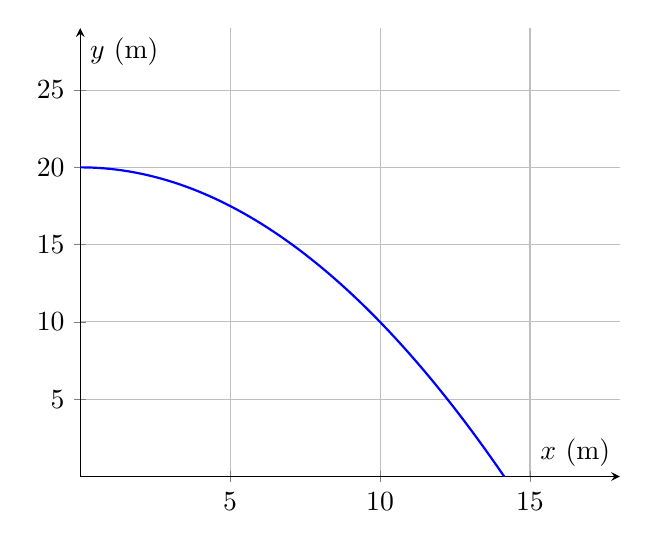
\begin{tikzpicture}
    \begin{axis}[
        xlabel={$x$ (m)},
        ylabel={$y$ (m)},
        xmin=0, xmax=18,
        ymin=0, ymax=29,
        axis x line=middle,
        axis y line=middle,
        grid=major,
        samples=100,
        domain=0:20,
    ]

    % Plot the trajectory y(x)
    \addplot[
        blue,
        thick
    ] {20 - (1 / 10) * x ^ 2};

    \end{axis}
\end{tikzpicture}

\documentclass{standalone}
\usepackage{pgfplots}
\pgfplotsset{compat=1.18}

\begin{document}

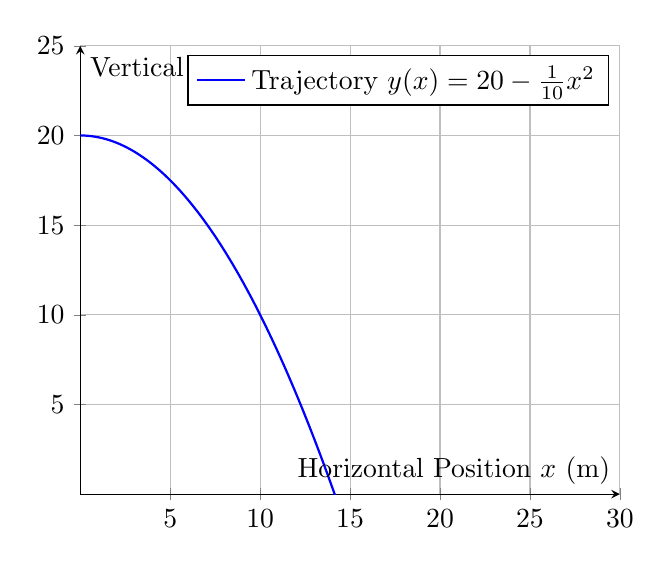
\begin{tikzpicture}
    \begin{axis}[
        xlabel={Horizontal Position $x$ (m)},
        ylabel={Vertical Position $y$ (m)},
        xmin=0, xmax=30,
        ymin=0, ymax=25,
        axis x line=middle,
        axis y line=middle,
        grid=major,
        samples=100,
        domain=0:20,
    ]

    % Plot the trajectory y(x)
    \addplot[
        blue,
        thick
    ] {20 - (1/10)*x^2};
    
    \addlegendentry{Trajectory $y(x) = 20 - \frac{1}{10}x^2$}
    
    \end{axis}
\end{tikzpicture}

\end{document}

xxx

\vfill
\subsection*{ANSWER}
\begin{enumerate}
    \item 1
    \item 2
\end{enumerate}